\documentclass[aspectratio=169]{beamer}
% \documentclass[12pt,t]{beamer}
% \usepackage[T1]{fontenc}
% \usepackage[charter,cal=cmcal]{mathdesign}
% \usefonttheme{professionalfonts}
\usetheme{OU}


\usepackage{silence}
\WarningsOff*

\newcommand{\orcid}[1]{\href{https://orcid.org/#1}{\textcolor[HTML]{A6CE39}{\aiOrcid}}}

\usepackage{hyperref}
\usepackage{academicons}
\usepackage{xcolor}
% \usepackage{csquotes}
% \usepackage{epigraph} 

\usepackage{tcolorbox}
\usepackage{adjustbox}
\usepackage{amsmath}
\usepackage{subcaption}
\usepackage{fontawesome5}
% \usepackage[dutch]{babel} % Dutch text; e.g. accents, hyphenation
% \usepackage[english]{babel} % English text; e.g. accents, hyphenation
\usepackage[british]{babel}

% \usepackage{listings} % to write program code
\usepackage{hyperref} % URLs; e.g. \url{...}
\usepackage{mathtools} % to write above arrow
% \usepackage{listings}

% \usepackage[cache=false]{minted}
% \usemintedstyle{friendly}
% \setminted[python]{frame=lines,framesep=2mm}
% \setminted[java]{frame=lines,framesep=2mm}
% \setminted[sql]{frame=lines,framesep=2mm}

\usepackage[style=ieee,backend=biber,doi=false,isbn=false,url=false,eprint=false]{biblatex}
\bibliography{presentation}
\AtBeginBibliography{\tiny}
\setbeamertemplate{bibliography entry title}{}
\setbeamertemplate{bibliography entry location}{}
\setbeamertemplate{bibliography entry note}{}
\setbeamertemplate{bibliography entry url}{}

\usepackage{ragged2e}


\title{From Rationalism to Empiricism in Software Testing Education Through Gamification}
\subtitle{INTED 2024}
\author{Niels Doorn \orcid{0000-0002-0680-4443} \and Tanja E.J. Vos \orcid{0000-0002-6003-9113} \and Beatriz Marín \orcid{0000-0001-8025-0023}}
\date{2024-3-4}

\begin{document}
\setbeamerfont{footnote}{size=\Tiny}
\setbeamerfont{caption}{size=\Tiny}
\setbeamertemplate{background canvas}[title frame 169]

\begin{frame}[noframenumbering,plain]
  \titlepage
\end{frame}

% \setbeamertemplate{background canvas}[ou chess]
% \begin{frame}[noframenumbering,plain]{Table of Contents}
%   \tableofcontents[hideallsubsections]
% \end{frame}

\section{Opening}

\setbeamertemplate{background canvas}[ou plain]
\setbeamertemplate{footline}[left frame number small logo]

\section{Introduction}

\setbeamertemplate{background canvas}[ou plain]

\begin{frame}{Importance of software testing}
\begin{figure}
    \centering
    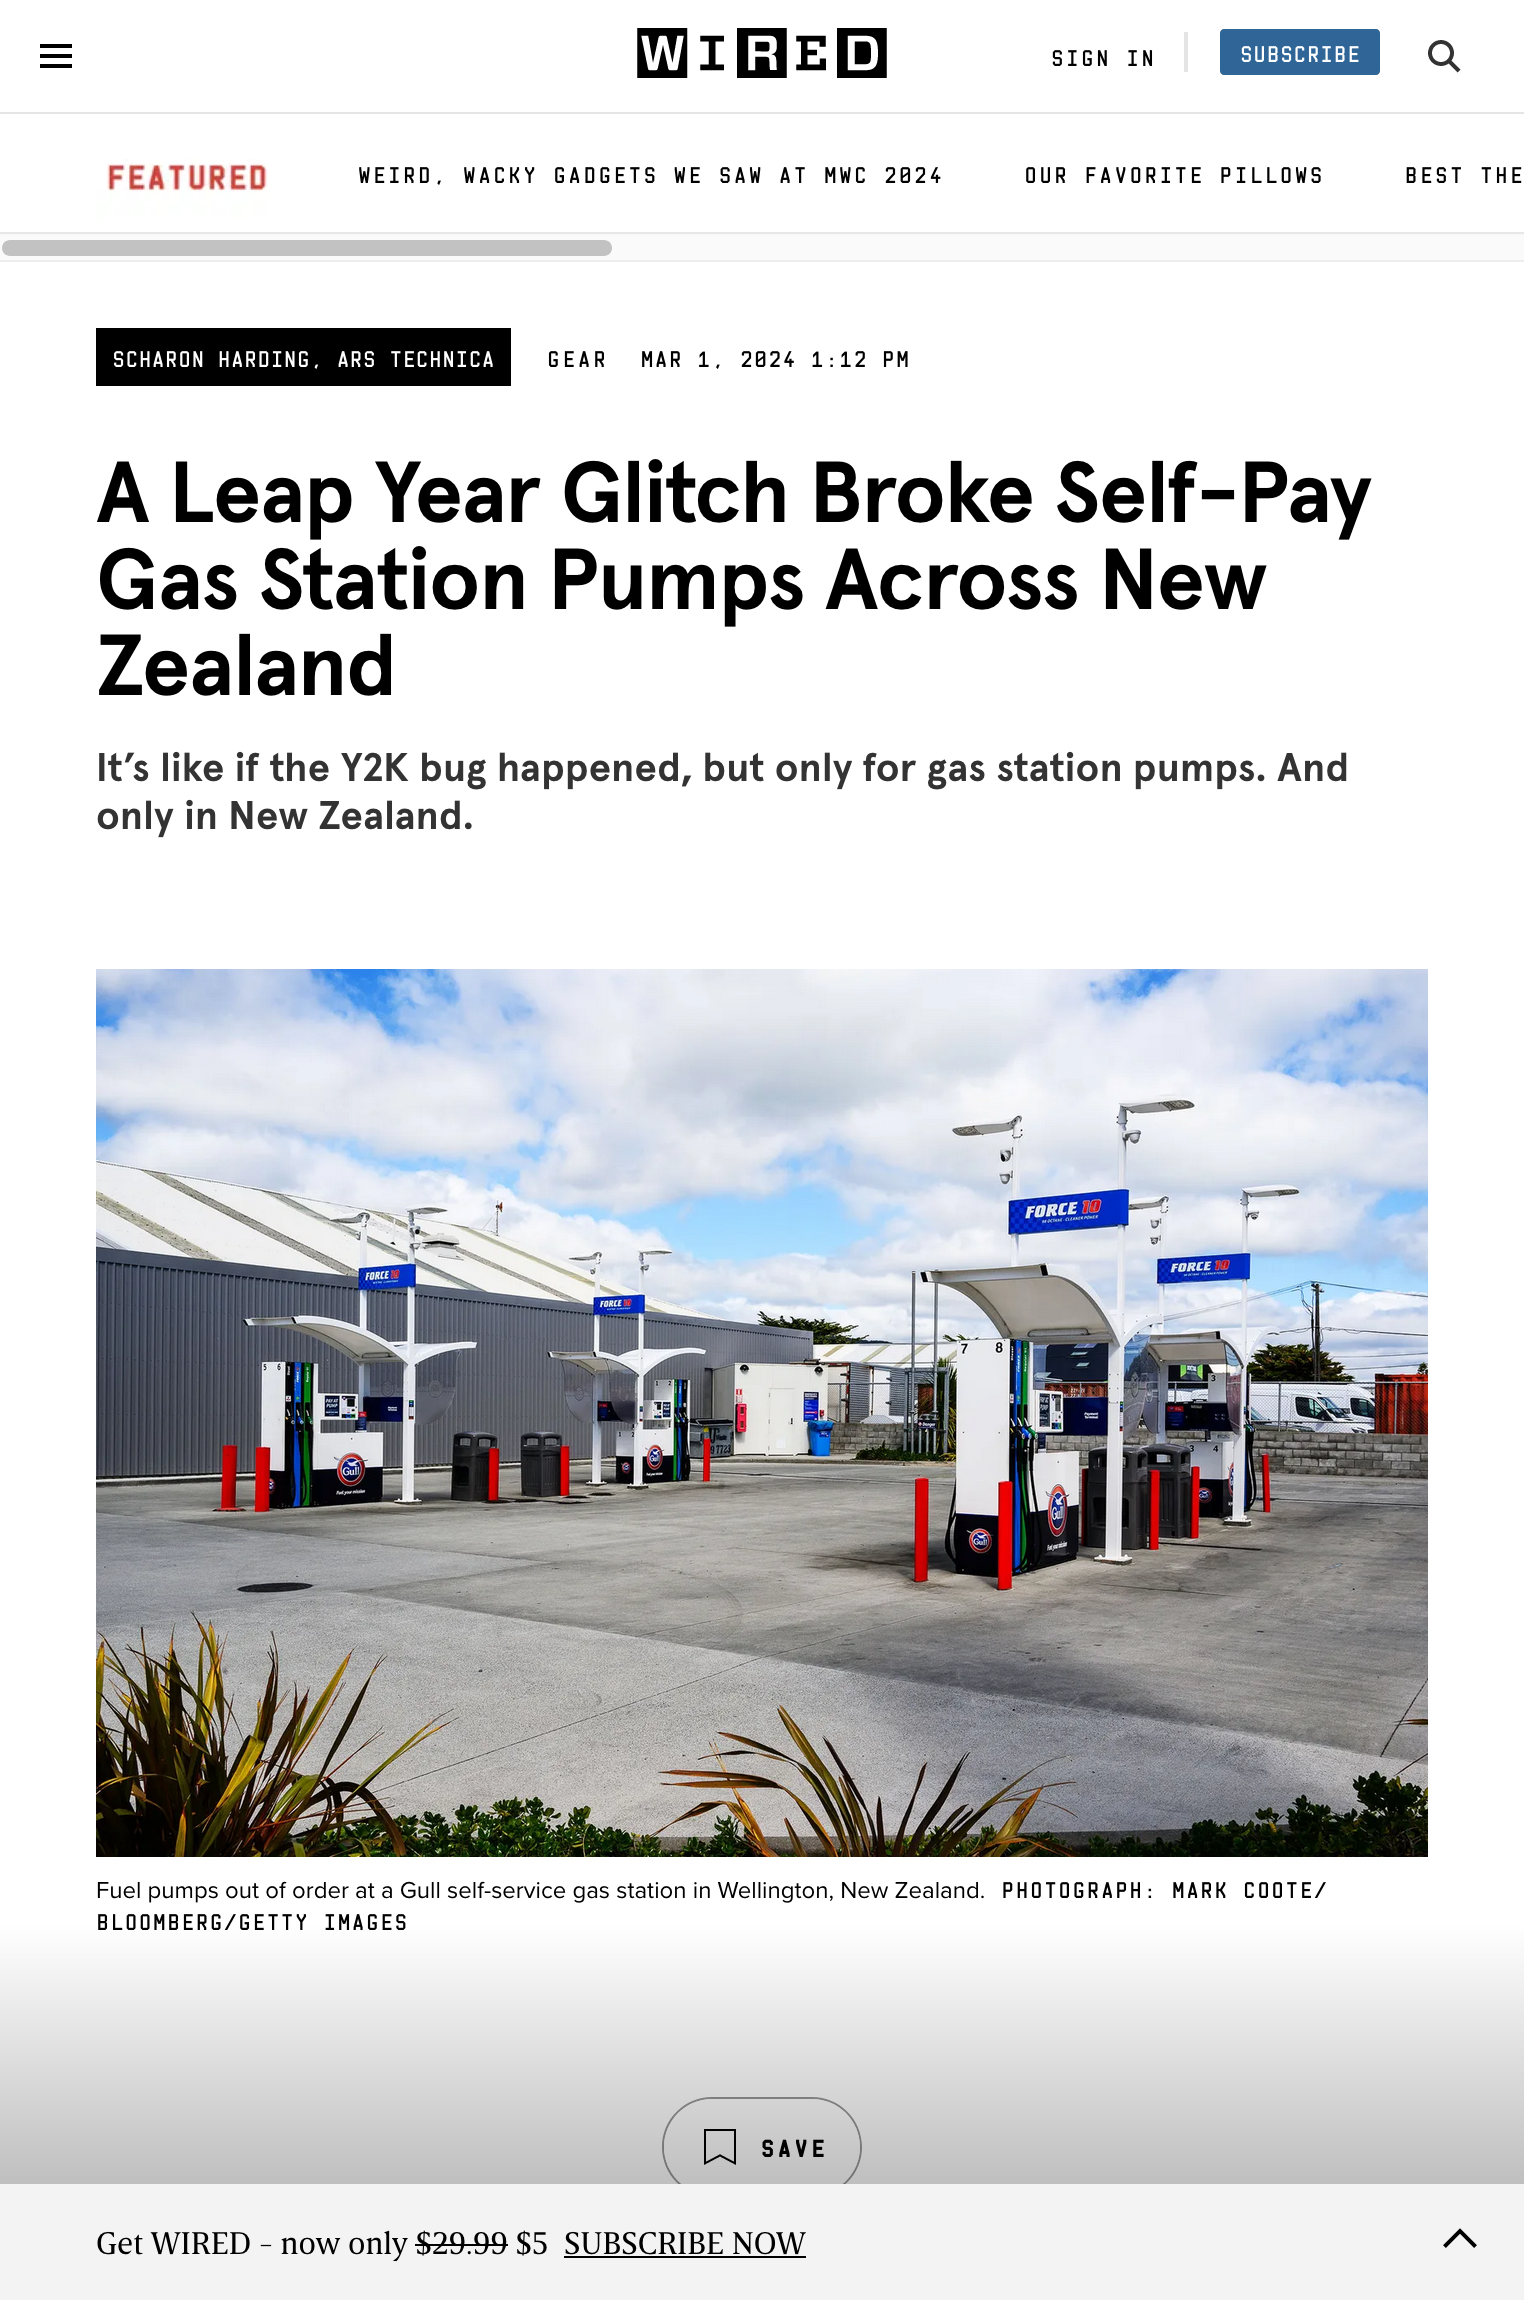
\includegraphics[width=0.9\linewidth]{images/bug.png}
    \caption{Screenshot of an article titled ``A Leap Year Glitch Broke Self-Pay Gas Station Pumps Across New Zealand''~\cite{ScharonHarding2024Mar}}
\end{figure}
\end{frame}

\begin{frame}{Software Testing in CS Education}
\begin{itemize}
    \item Integrating it into Computer Science curricula is challenging~\cite{garousi2020software, scatalon2020teaching}.
    \item Often a \textbf{rational design paradigm} is used in CS programs.
    % \item We need to shift to a design paradigm based on empiricism.
    \item Little research on didactic approaches is available.%, we think an approach based on abductive reasoning works.
    % \item In general, the use of serious games can be helpful.
    % \item We hypothesize that combining gamification with Socratic questioning can significantly improve the learning of software testing.
    % , fostering a shift towards an empirical design paradigm that emphasizes reflection-in-action and critical thinking.
    % \item We started with the development of a serious game.%, where students devise a testing strategy for a system under test.
    % \item We use Socratic questioning as innovative approaches to enhance software testing education. 
    % These methods aim to foster engagement, practical application, immediate feedback, collaborative learning, and complex problem-solving.
\end{itemize}
\end{frame}

\begin{frame}{Consequences}
    The way we now teach software testing leads to:
    \begin{itemize}
        \item Students who use a `developer approach' to testing~\cite{doorn2023towards}.
        \item This approach lacks exploration and experimentation.
    \end{itemize}
    \vspace{1cm}
    We need to shift the mental model of students away from this rational approach.
\end{frame}

% \begin{frame}{How we should teach software testing}
%     \begin{itemize}
%         \item Prevalence of `developer approach' in testing by students.
%         \item We need to shift their mental model.
%         \item We need the right didactic approach.
%     \end{itemize}
% \end{frame}

\setbeamertemplate{background canvas}[ou plain]
\begin{frame}[noframenumbering,plain]
\begin{figure}
    \centering
    \vspace{-1cm}
    \hspace*{-1.2cm}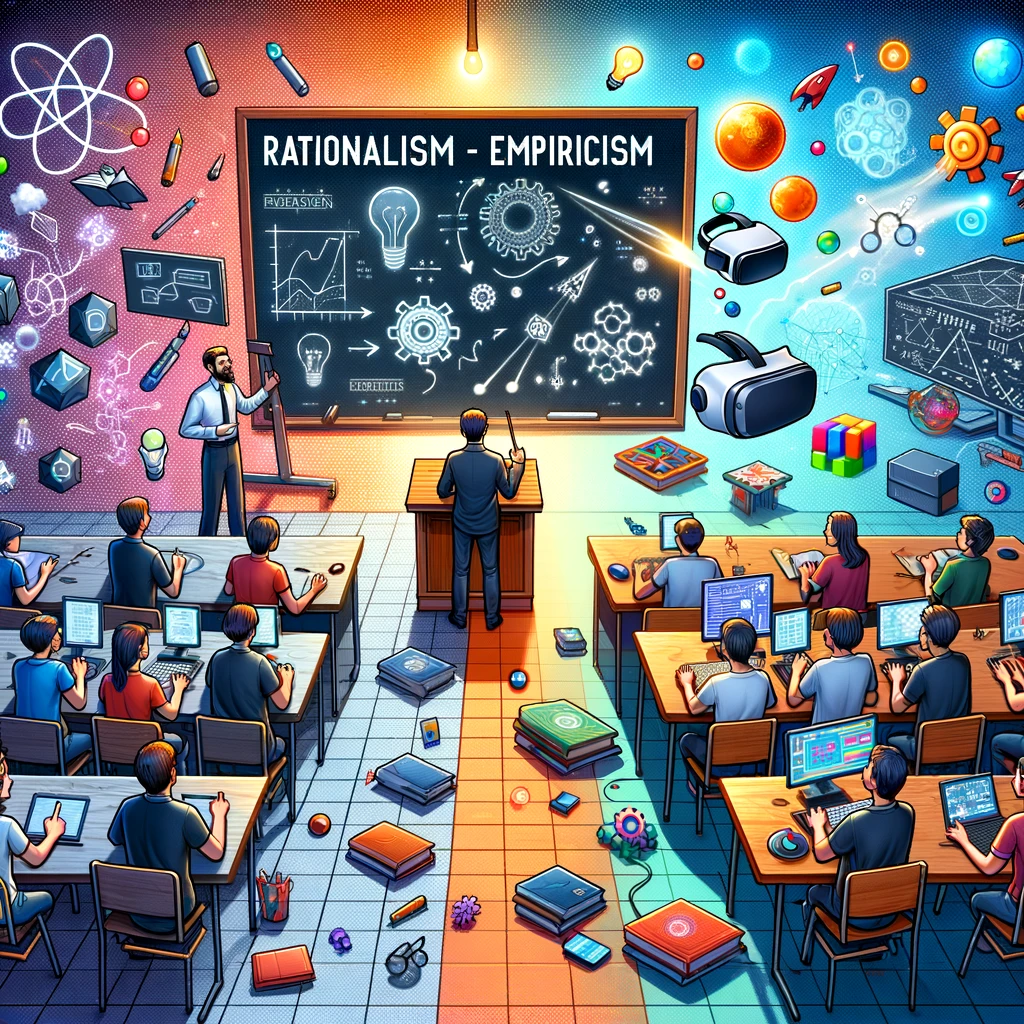
\includegraphics[width=1.2\linewidth]{images/plaatje.png}
\end{figure}
\end{frame}

% \begin{frame}{Shift to Empiricism}
%     \begin{itemize}
%         \item Need for an approach based on empiricism in teaching software testing.
%         \item Emphasis on experimentation and heuristic-based learning.
%         \item Students should follow an iterative process:
%         \begin{itemize}
%             \item form hypotheses based on observation and heuristics, 
%             \item design tests and execute them,
%             \item and analyse the feedback.
%         \end{itemize}
%     \end{itemize}
% \end{frame}

\begin{frame}{Abductive reasoning as the base for testing}
    Abductive reasoning is a form of logical inference that seeks the simplest and most likely conclusion from a set of observations~\cite{ContributorstoWikimediaprojects2024Feb}.
\end{frame}

\begin{frame}{Abductive reasoning as the base for testing}
    Abductive reasoning is a form of logical inference that seeks the simplest and most likely conclusion from a set of observations~\cite{ContributorstoWikimediaprojects2024Feb}.\\
    \vspace{0.5cm}
    This fits very well with exploratory testing because:\\
    \vspace{0.5cm}
    \textbf{What} the behaviour of the system looks like is unknown, \textbf{how} the design process of tests should look like is unknown. The \textbf{desired situation} is unknown, and so is \textbf{the road towards it}.
\end{frame}

% \begin{frame}{Didactics for software testing:\\Abductive Reasoning}
%     \begin{blockquote}
%     If it looks like a duck, and quacks like a duck, we have at least to consider the possibility that we have a small aquatic bird of the family Anatidae on our hands\\
%     \textit{-- Douglas Adams}~\cite{adams1987dirk}.
%     \end{blockquote}
% \end{frame}

% \begin{frame}{Didactics for software testing:\\Abductive Reasoning}
%     \textbf{What} the SUT should look like is unknown, \textbf{how} the design process of tests should look like is unknown. The \textbf{desired situation} is unknown, and so is the road towards it.
% \end{frame}

\section{Gamification in CS}

\setbeamertemplate{background canvas}[ou plain]
\begin{frame}{Development of a game to teach software testing}
    Our goals for a serious game:
    \begin{itemize}
        \item Incorporating empirical methods and critical thinking.
        \item Supporting different educational contexts.
        \item Enabling abductive reasoning.
    \end{itemize}
\end{frame}

\begin{frame}%[allowframebreaks]
    \frametitle{Gamification in CS}
    \begin{itemize}
        \item Gamification is effective in CS education through: Real-world scenarios, competitive elements, immediate feedback, interactive activities, and collaboration~\cite{8658524}.
        \item Gamification is applicable across various educational strategies and contexts~\cite{informatics9040075, hirsh2022, Tan_Chong_2023}.%, enhancing engagement in software measurement processes, software testing education, and integration of modern technology stacks.
        % \item Innovative tools and techniques include educational chatbots and the use of serious games in secure programming~\cite{10.1145/3350768.3352456,8802503}.
        % \item The educational impact and methodologies section discusses successful game-based interventions, methodologies for evaluating such interventions, and the Scrum Game Challenge for learning Scrum methodologies.
        \item Applying gamification can lead to oversimplification and decreased intrinsic motivation~\cite{8658524}.
        % \item Offline games such as TestSphere and `Would Heu-Risk It?' card games can enhance software testing discussions, collaboration, and strategy design~\cite{testsphere, BibEntry2023Sep}.
        % \item Methods like `The TestOpsy' and `Blackbox Puzzles' focus on the testing process and improving problem-solving skills~\cite{ChrisKenst2022Jun, BibEntry2022Feb}.
        % \item A systematic review on game-based learning's impact on argumentation skills emphasizes the importance of game elements, instructional supports, and learning theories for enhancing argumentation skills through game-based environments.
        % \item Specific games such as `Testable', `Testing Maze', `CleanGame', and 'Code Defenders' are designed to improve aspects like unit testing, functional testing, code smell identification, and mutation testing~\cite{8994972,10.1145/3613372.3614191,10.1145/3350768.3352490,10.1145/3287324.3287471,9155973}.
    \end{itemize}
\end{frame}

\begin{frame}{CodeDefenders: game to learn mutation testing}
\begin{figure}
    \centering
    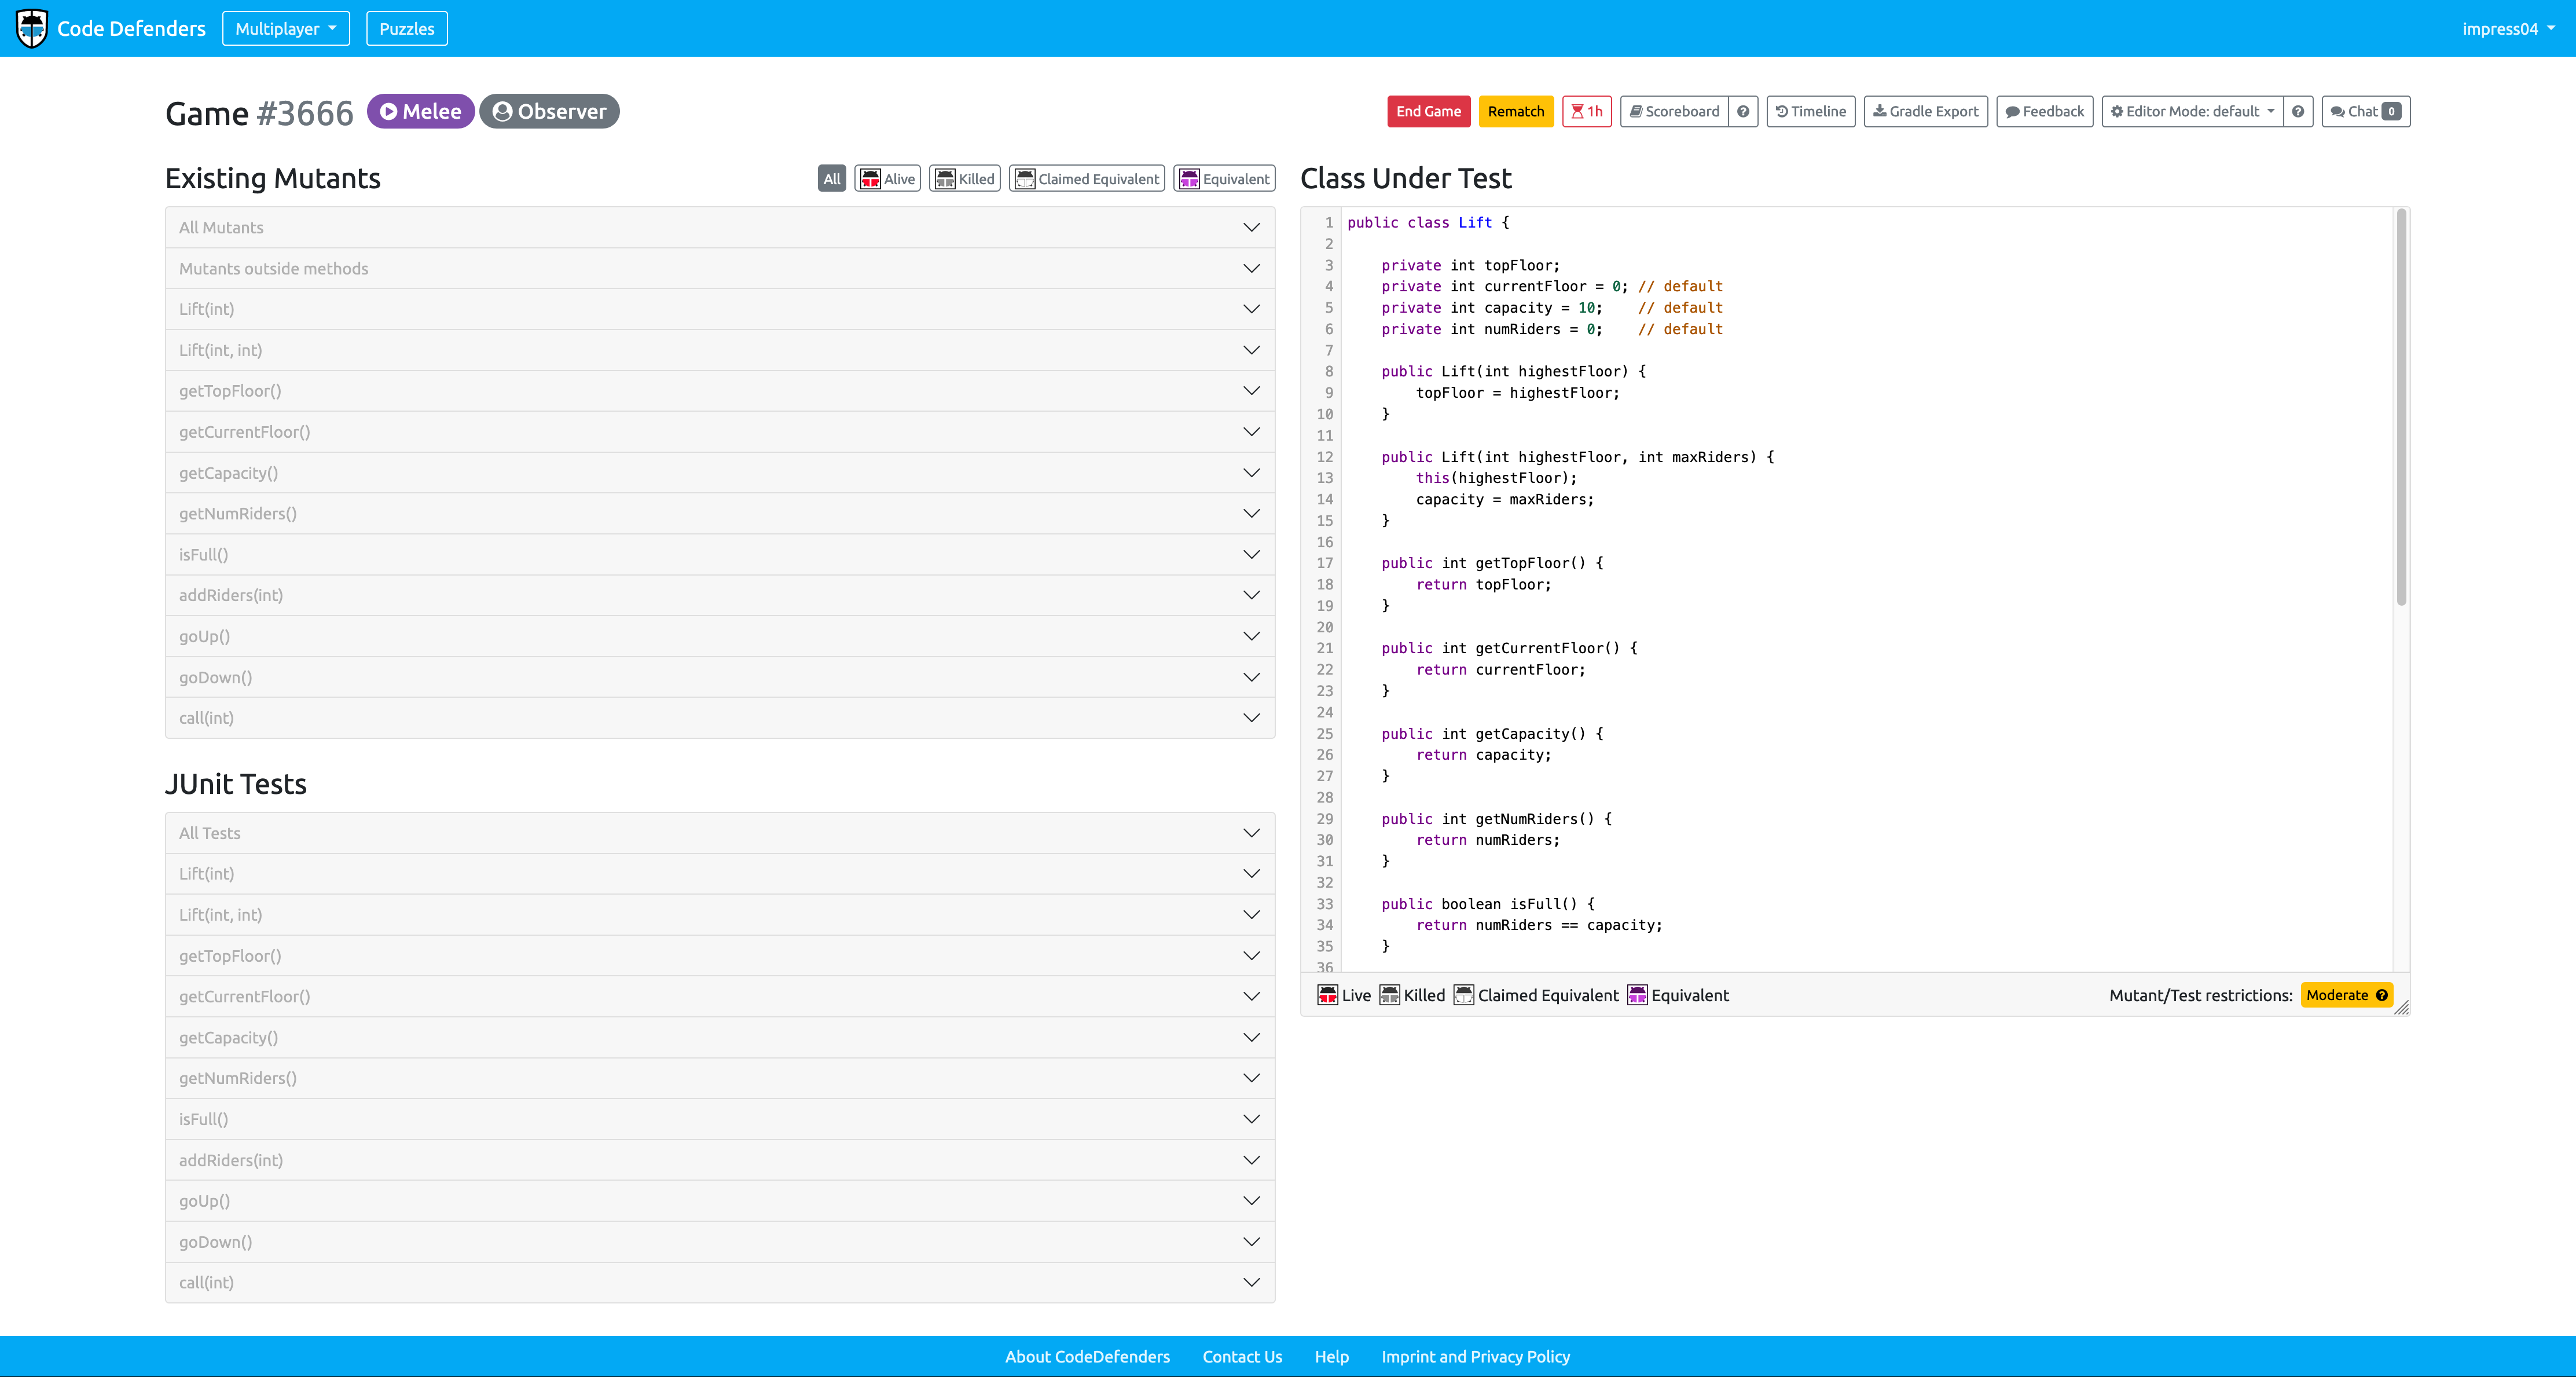
\includegraphics[width=0.75\linewidth]{images//games/codedefenders.png}
    \caption{CodeDefenders, an online game to learn mutation testing}
\end{figure}
\end{frame}

\begin{frame}{Testable: gamification of unit testing}
\begin{figure}
    \centering
    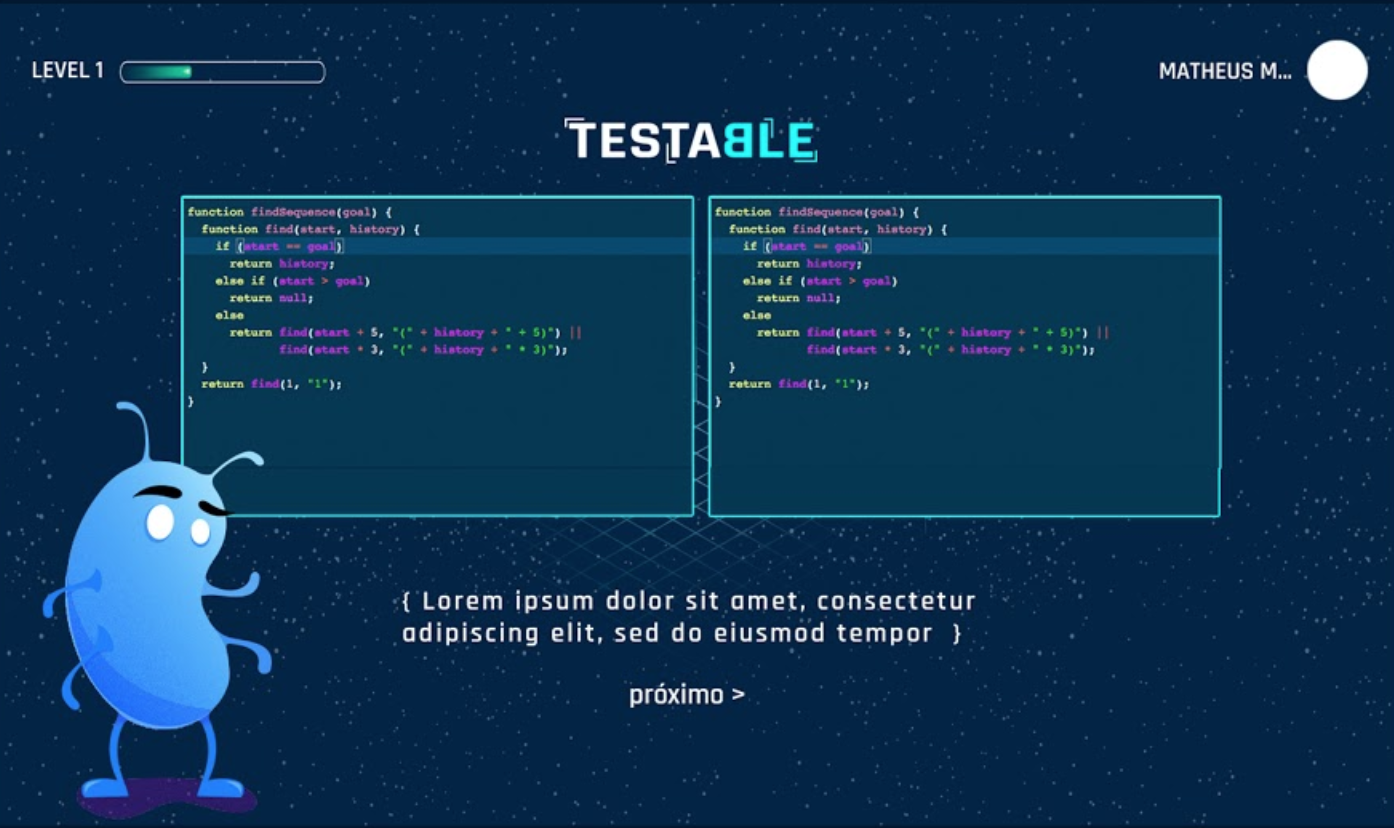
\includegraphics[width=0.75\linewidth]{images//games/testable}
    \caption{Testable - gamified tool to improve unit testing teaching}
\end{figure}
\end{frame}

\begin{frame}{Testing Maze: adventure into functional testing}
\begin{figure}
    \centering
    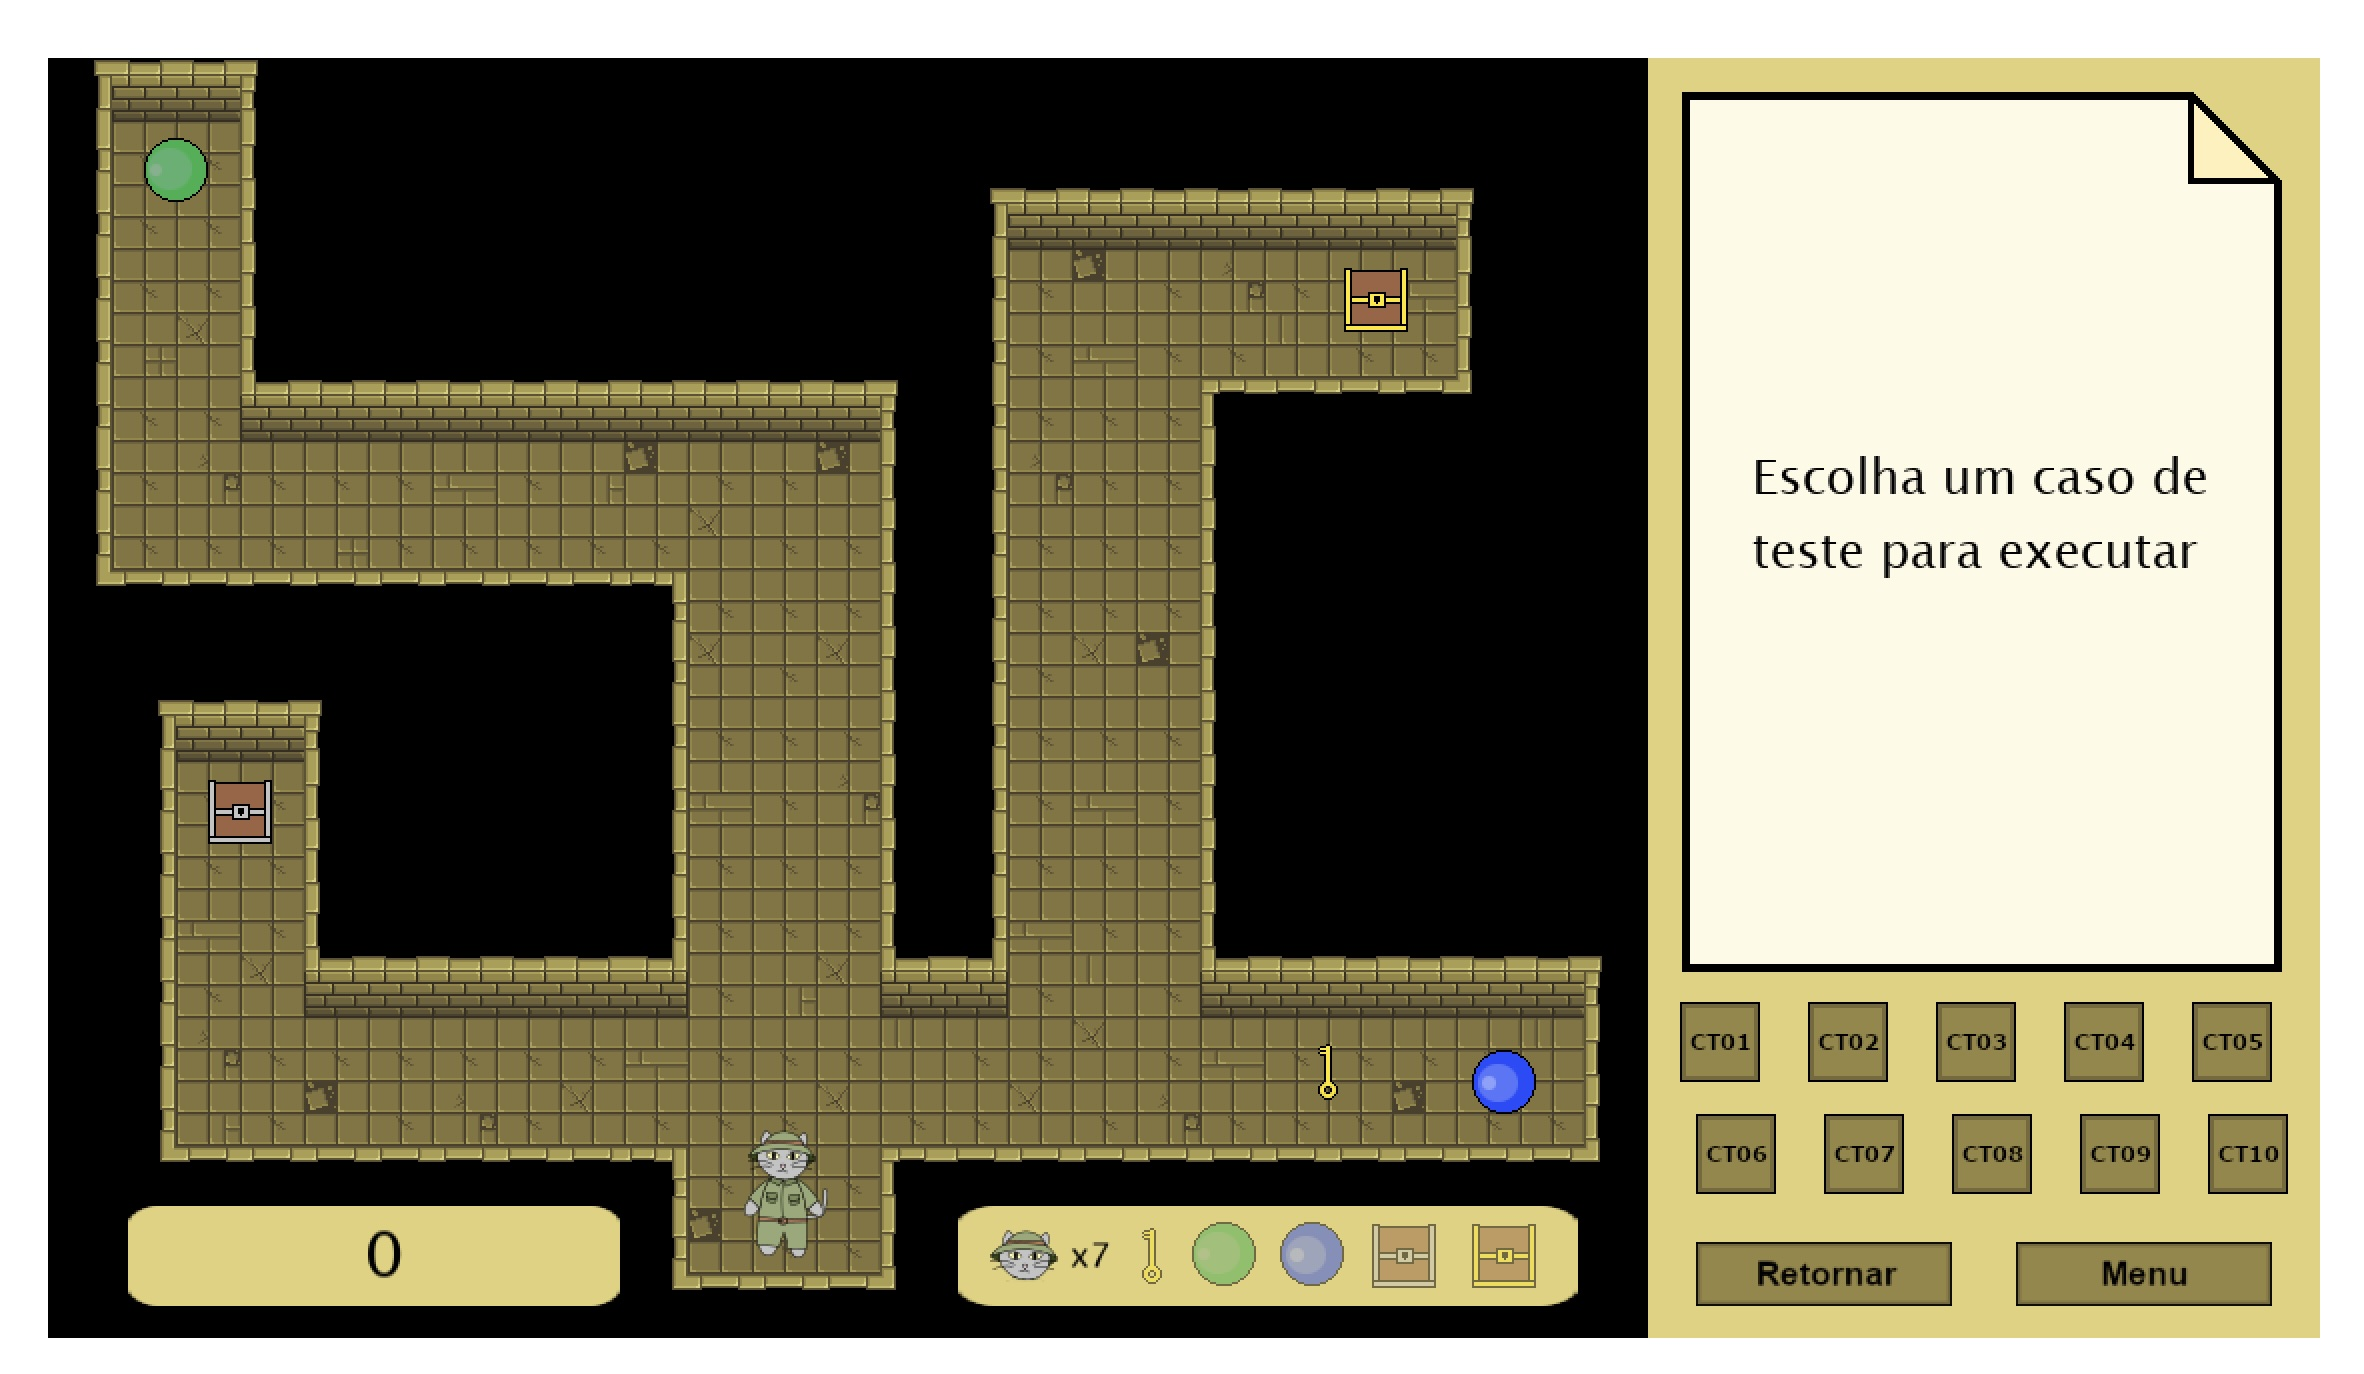
\includegraphics[width=0.75\linewidth]{images//games/testingmaze}
    \caption{Testing Maze, an educational puzzle game for teaching functional testing concepts and test specifications containing a fantasy narrative}
\end{figure}
\end{frame}

\begin{frame}{TestSphere: card deck to support interaction}
\begin{figure}
    \centering
    
\includegraphics[width=0.5\linewidth]{images//games/testsphere}
    \caption{TestSphere, a card deck to support testers thinking and talking about testing}
\end{figure}
\end{frame}

\begin{frame}{Would Heu-risk it?: card deck to share experiences}
\begin{figure}
    \centering
    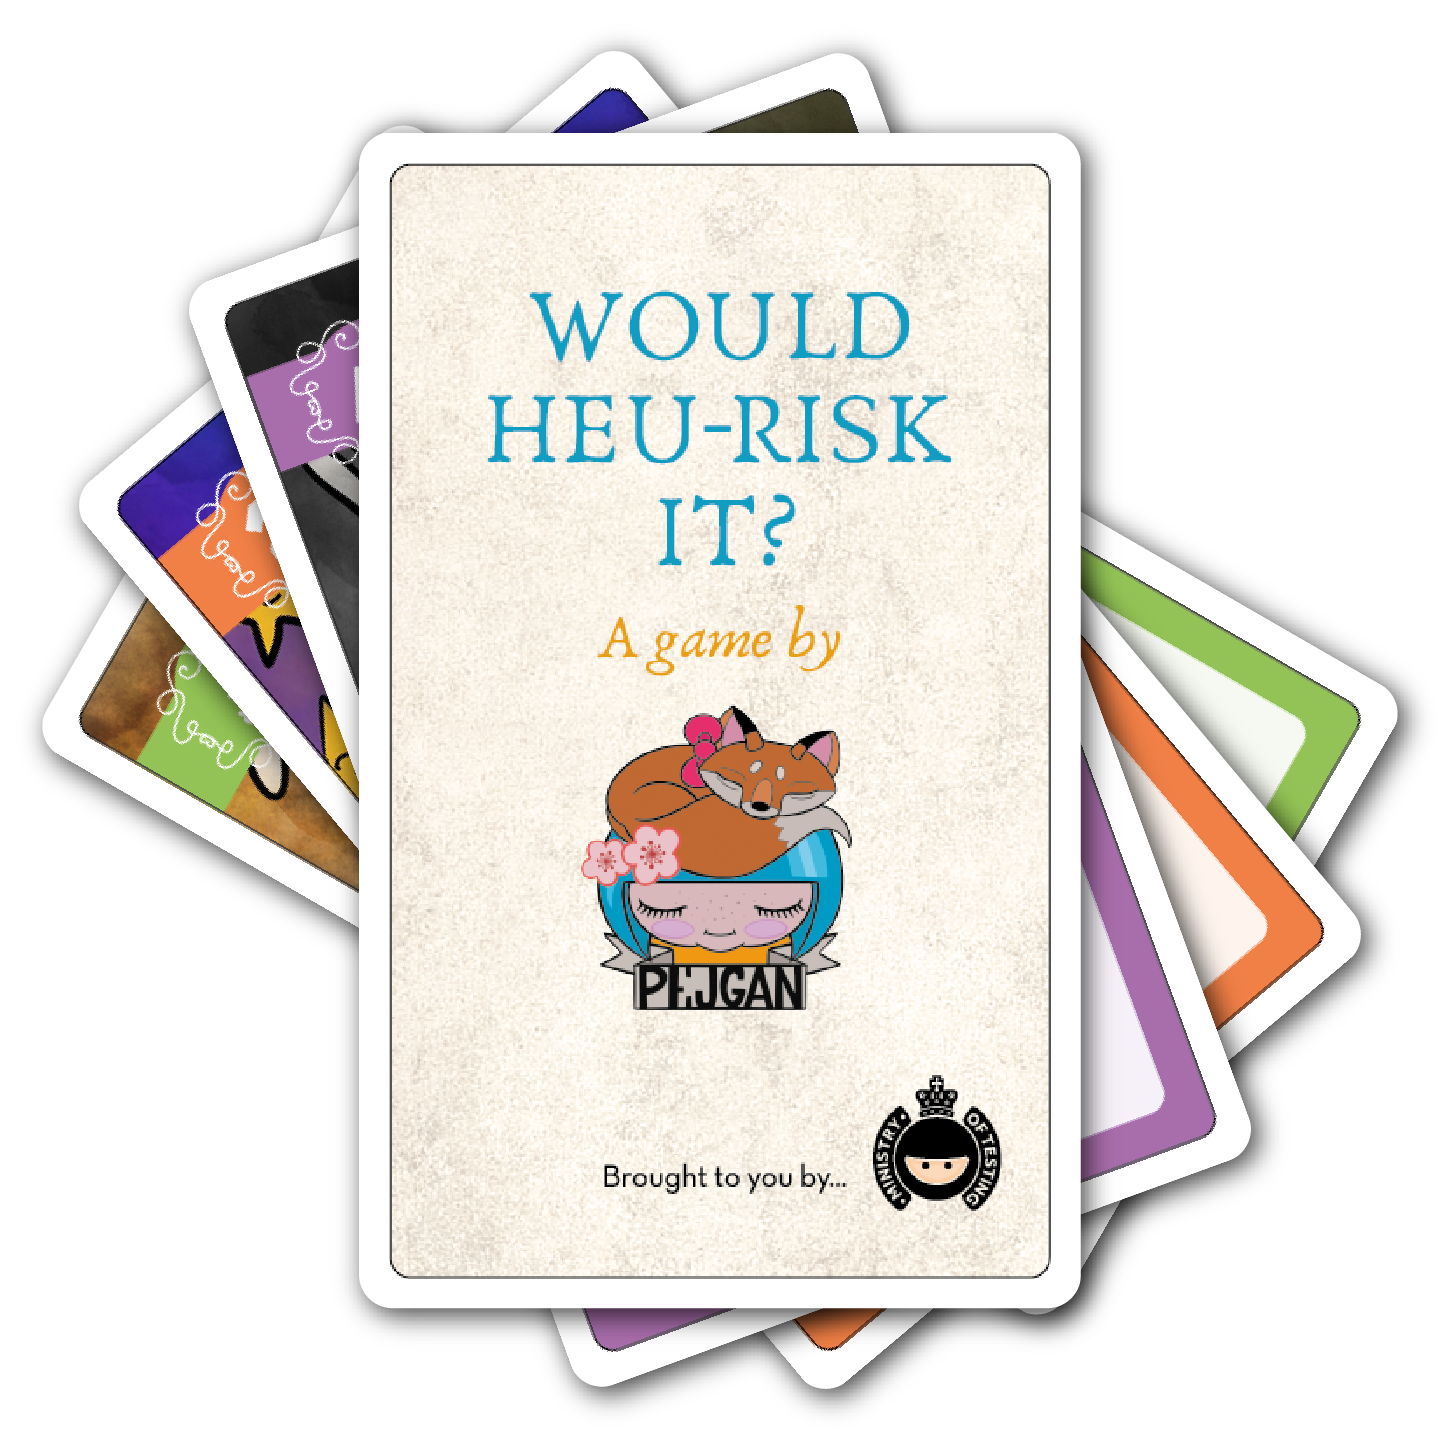
\includegraphics[width=0.5\linewidth]{images//games/would}
    \caption{`Would Heu-risk it?' is centered around risk analysis, heuristics, patterns/anti-patterns of software testing}
\end{figure}
\end{frame}

\begin{frame}{Gap in existing game and our goals}
    \begin{itemize}
        \item Most games focus on techniques.
        \item No games on our goals.
        \item We need to develop a game ourselves.
    \end{itemize}
\end{frame}

\begin{frame}{Our game}
    Based on Risk Storming using TestSphere:
    \begin{enumerate}
        \item Starting with a System Under Test.
        \item Identifying thee most relevant quality aspects.
        \item Identifying risks for these aspects, \textbf{supported by socrative questions}.
        \item Mitigate these risks with techniques.
        \item Form an initial testing plan.
    \end{enumerate}
\end{frame}

\begin{frame}{Socrative Questioning}
    Socratic questions are a form of inquiry and discussion between individuals, based on asking and answering questions to stimulate critical thinking and to illuminate ideas.
\end{frame}

\begin{frame}{Examples of Socrative Questions used in the game}
    \begin{itemize}
        \item How does the system verify and ensure that the data processed is current and accurate?
        \item In what ways does the system maintain the confidentiality and integrity of personal data?
        \item Are there any performance benchmarks or metrics that the system is expected to meet?
        \item What are the disaster recovery and business continuity plans for the system?
    \end{itemize}
\end{frame}

\begin{frame}{Wheel of socrative questions}
    \begin{figure}
        \centering
        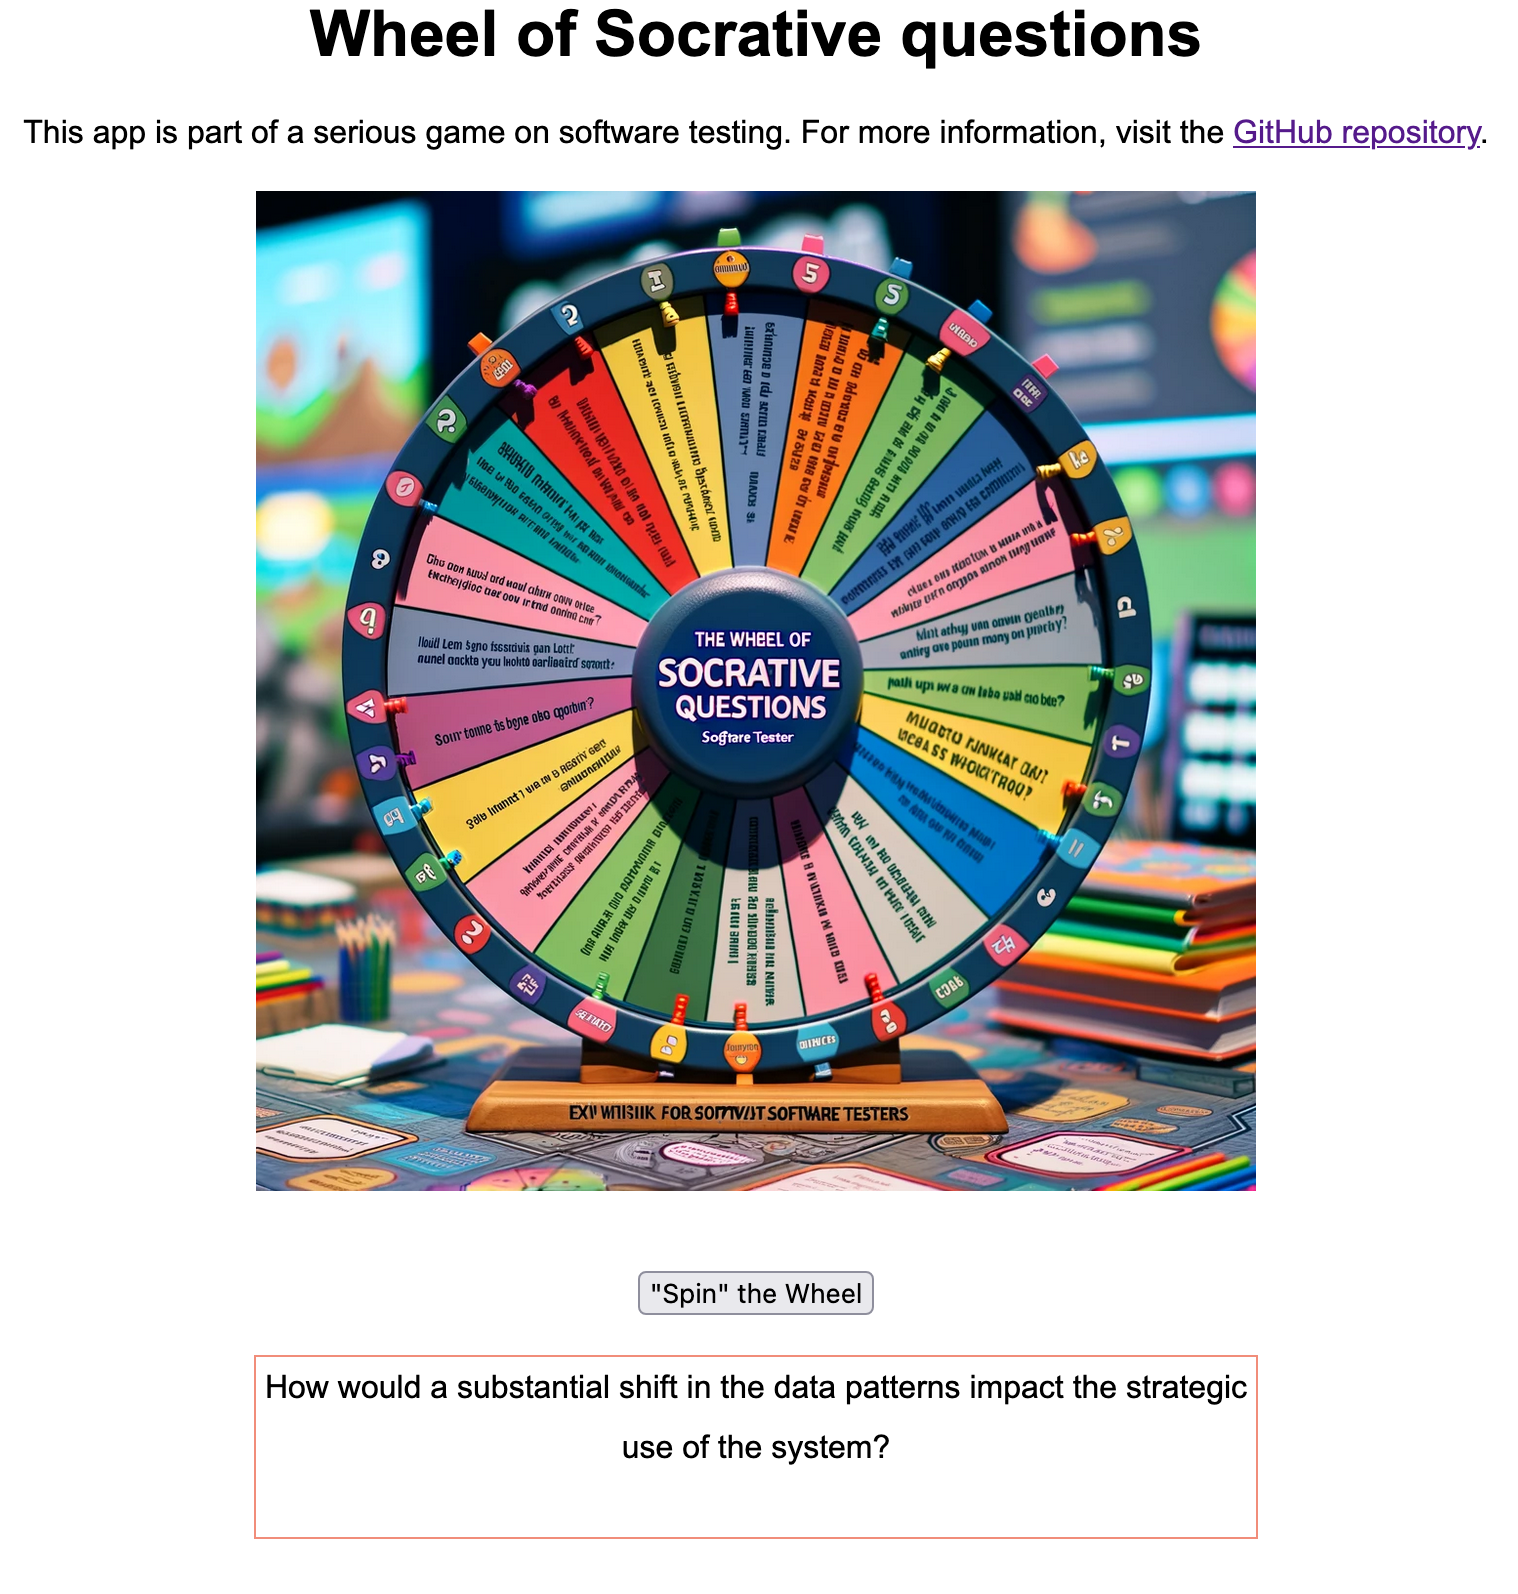
\includegraphics[width=0.5\linewidth]{images//wheel}
        \caption{"The Wheel of Socrative Questions," a game wheel designed for software testers}
    \end{figure}
\end{frame}

\begin{frame}{Pilot Study \& Results}
    \begin{itemize}
        \item We did a pilot study with four sessions with Bachelor and Master CS students of OU an NHL Stenden.
        \item Improvements observed in students' testing strategies.
        \item Student's feel more secure about their tests.
    \end{itemize}
\end{frame}

\begin{frame}{Pilot Study \& Results}
    \begin{figure}
        \centering
        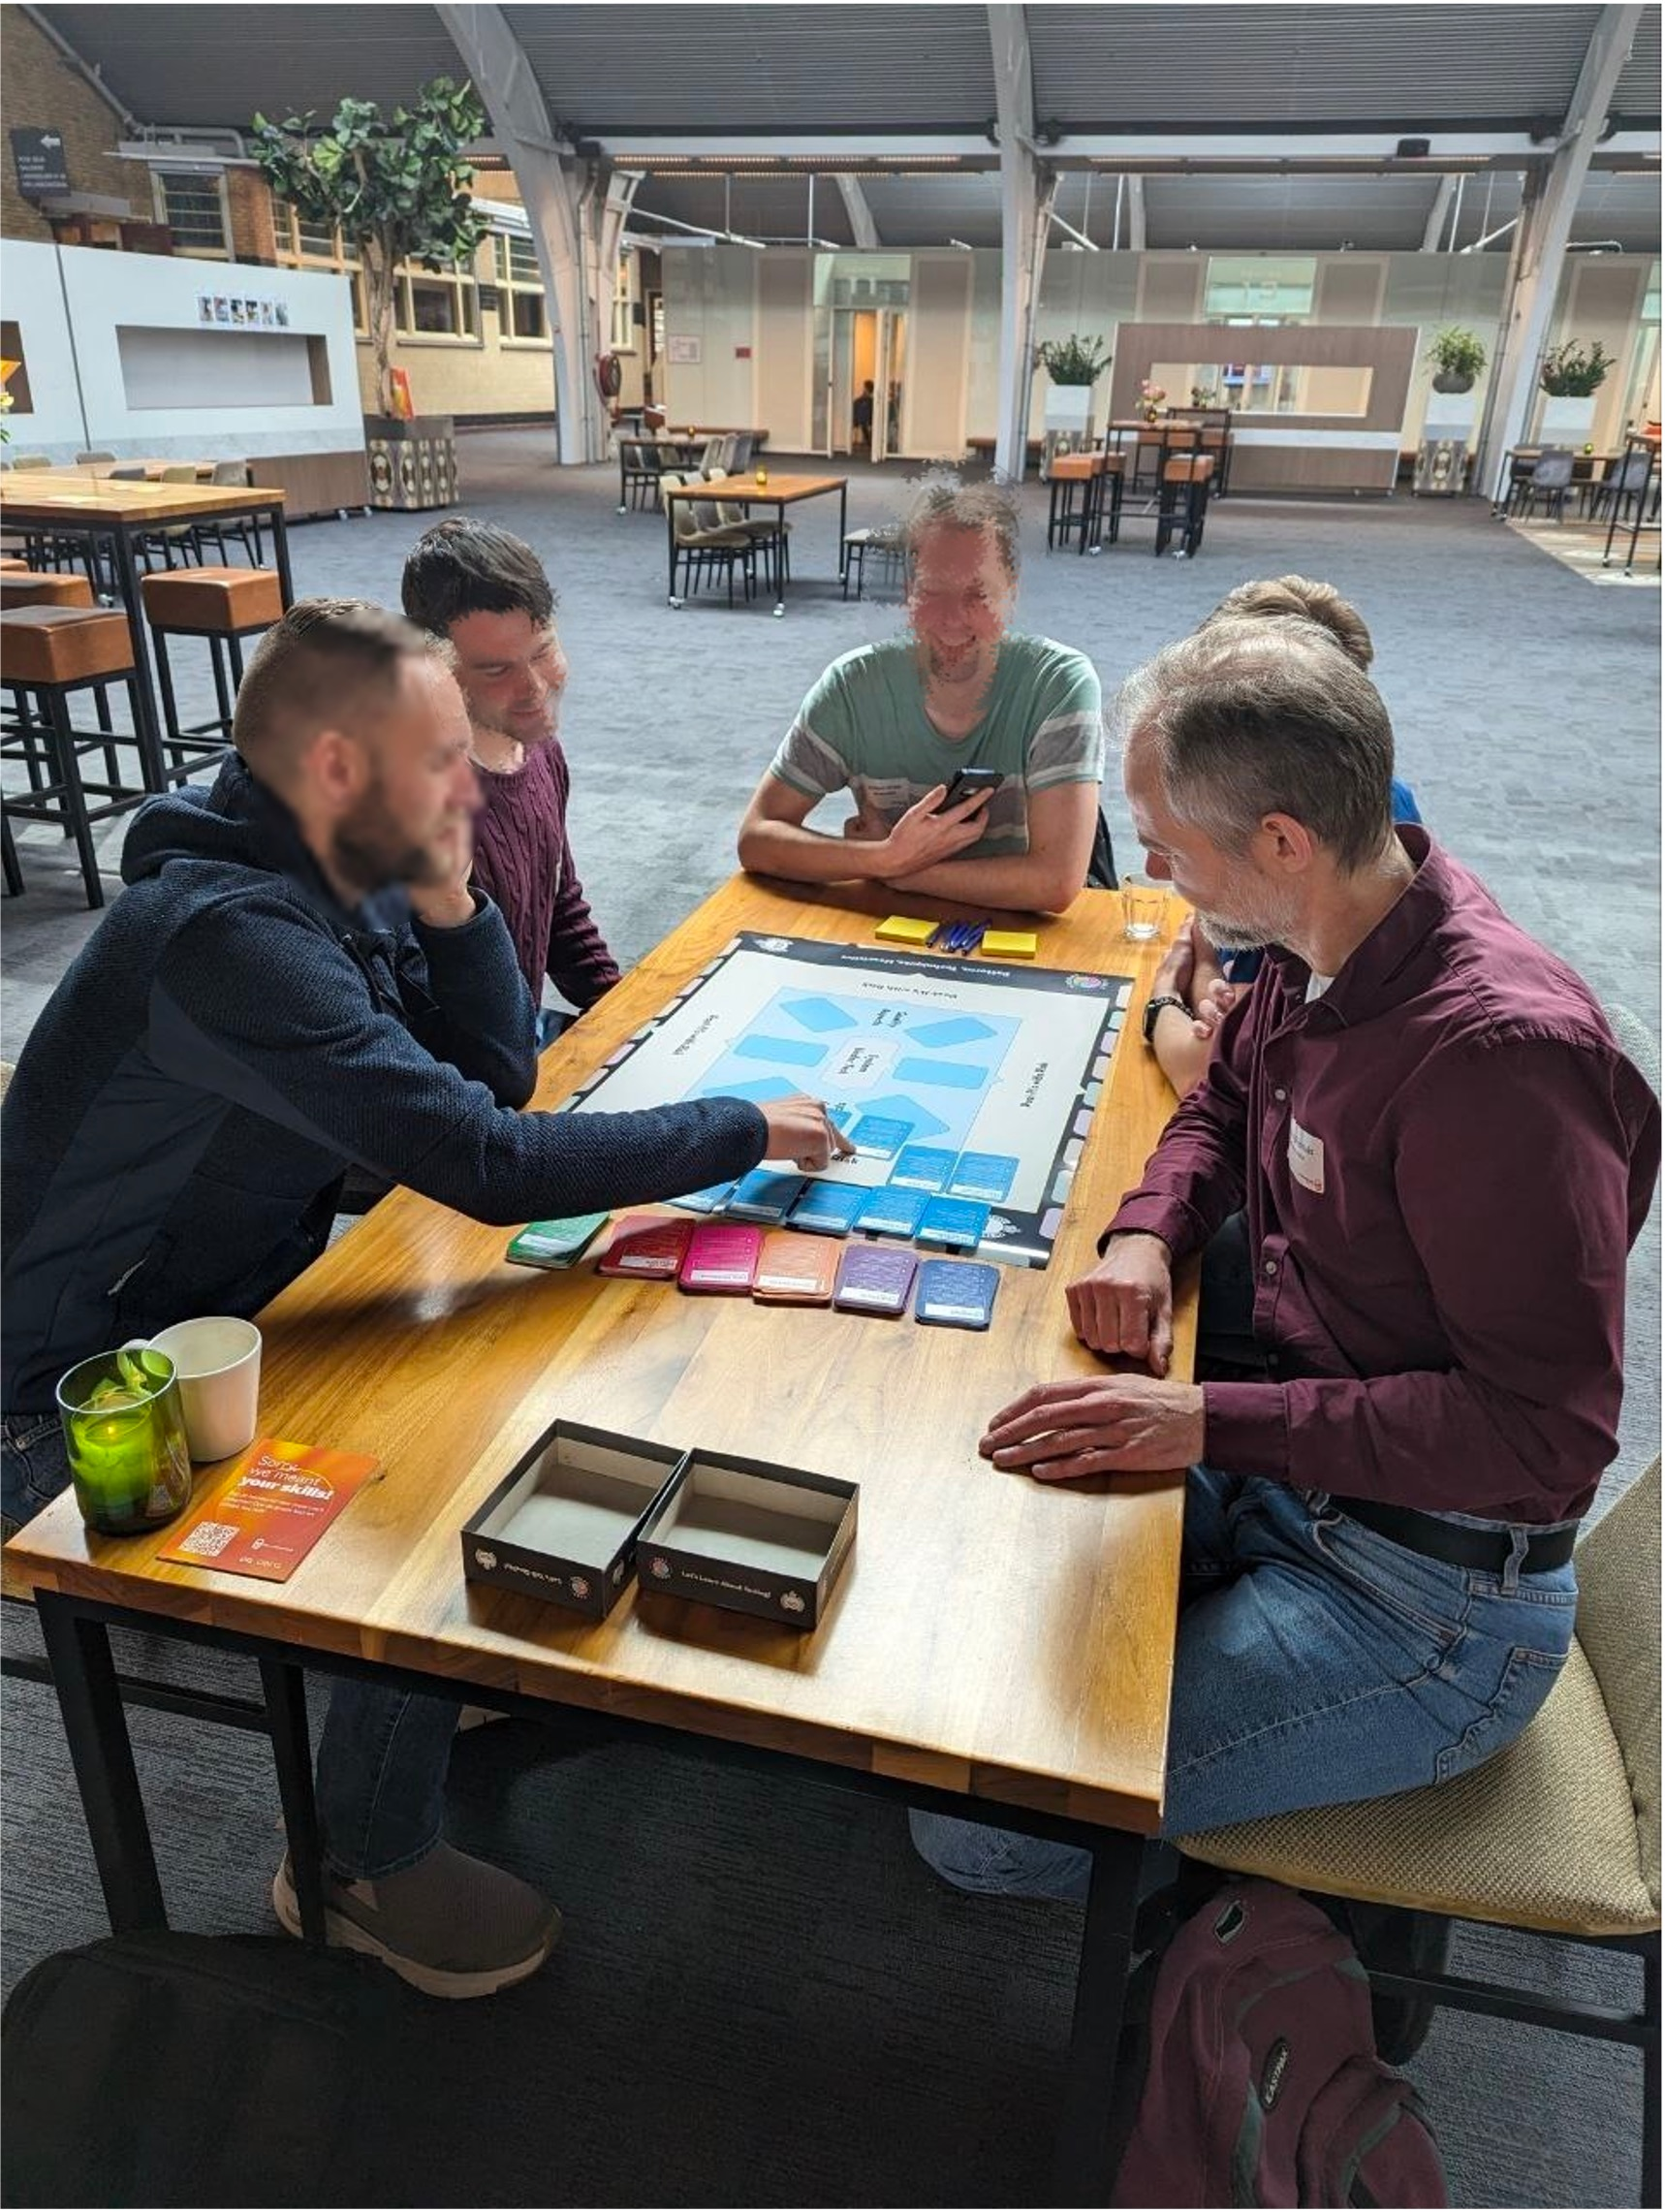
\includegraphics[width=0.4\linewidth]{images//Imagen1.jpg}
        \caption{Students playing the game}
    \end{figure}
\end{frame}

\section{Future work}

\setbeamertemplate{background canvas}[ou plain]
\begin{frame}{Future Work}
    \begin{itemize}
        \item Further develop game mechanics.
        \item Validate and expand the socratic questions.
        \item Trials with students in different educational contexts.
        \item Publish the game (under CC license).
    \end{itemize}
\end{frame}

\section{Conclusion and thanks}

% \setbeamertemplate{background canvas}[ou birds]
% \begin{frame}{Conclusion}
%     \begin{itemize}
%         \item Summary of the shift towards an empirical approach.
%         \item Potential impact on software testing education.
%     \end{itemize}
% \end{frame}

\setbeamertemplate{background canvas}[ou plain]
\begin{frame}{Thanks for your attention}

% \begin{flushright}
% \vspace{2cm}
% \begin{minipage}{6cm}
\begin{itemize}
    \item Software Testing is important.
    \item We need to shift to an approach based on empiricism.
    \item Gamification is an approach to support this in multiple educational contexts.
    \item We propose abductive reasoning as a basis for the didactic approach.
    \item We did a pilot to gain insights using socrative questioning.
    \item Game mechanics need to be further developed.
\end{itemize}

% \end{minipage}
% \end{flushright}

\begin{figure}
    \centering
    
\includegraphics[width=0.25\linewidth]{images//qr.png}
    \caption{More information about my research on \url{https://research.nielsdoorn.nl}}
\end{figure}
\end{frame}

\setbeamertemplate{background canvas}[ou plain]
\begin{frame}{Acknowledgements}
    This work was funded by the ENACTEST -- European innovation alliance for testing education (ERASMUS+ Project number 101055874, 2022-2025). %And Kimmie, for her support when I needed it most. And her feedback on the game, basically, it was all her idea.
\end{frame}

\setbeamertemplate{background canvas}[ou plain]
\begin{frame}[allowframebreaks]
    \frametitle{References}
    \printbibliography
\end{frame}

\end{document}
